Yvonne Coady will be the executive in charge of the entire network:
the setting and meeting of short-term goals and the general financial
planning.  The bulk of the software will be developed at UVic, under
her supervision. She will be in charge of hiring and managing the team
to develop the knowledge-transformation platform. She will also design
the general architecture of CHORUS.

Jeremy Heyl will engage the core group of stakeholders and grow the
network to new domains.  The initial domains are remote sensing,
geosciences, public health and archaeology.  He has already contacted
additional potential collaborators in forestry and fisheries, and will
develop contacts in other areas of natural resources and social
sciences.  Jeremy will be in charge of the organization of the formal
collaboration meetings as well as the team meetings within the
individual domains to discuss their detailed needs and incorporate
them into the software development. He will gather the contributions
from the individual stakeholders, identifying which databases to
include and how to include them.  He will also design the initial set
of analysis tools available within the platform and will develop the
interface in collaboration with partners at STSci and Magnetar Games.

We have identified key stakeholders in several initiual areas.  Each
of them will identify further stakeholders within their area to
discover the market within their area and subsequently they will
engage the stakeholders within their area to identify their needs
(market validation).  They will also interface with the software
development team to help create prototypes (productization).

\begin{figure}
  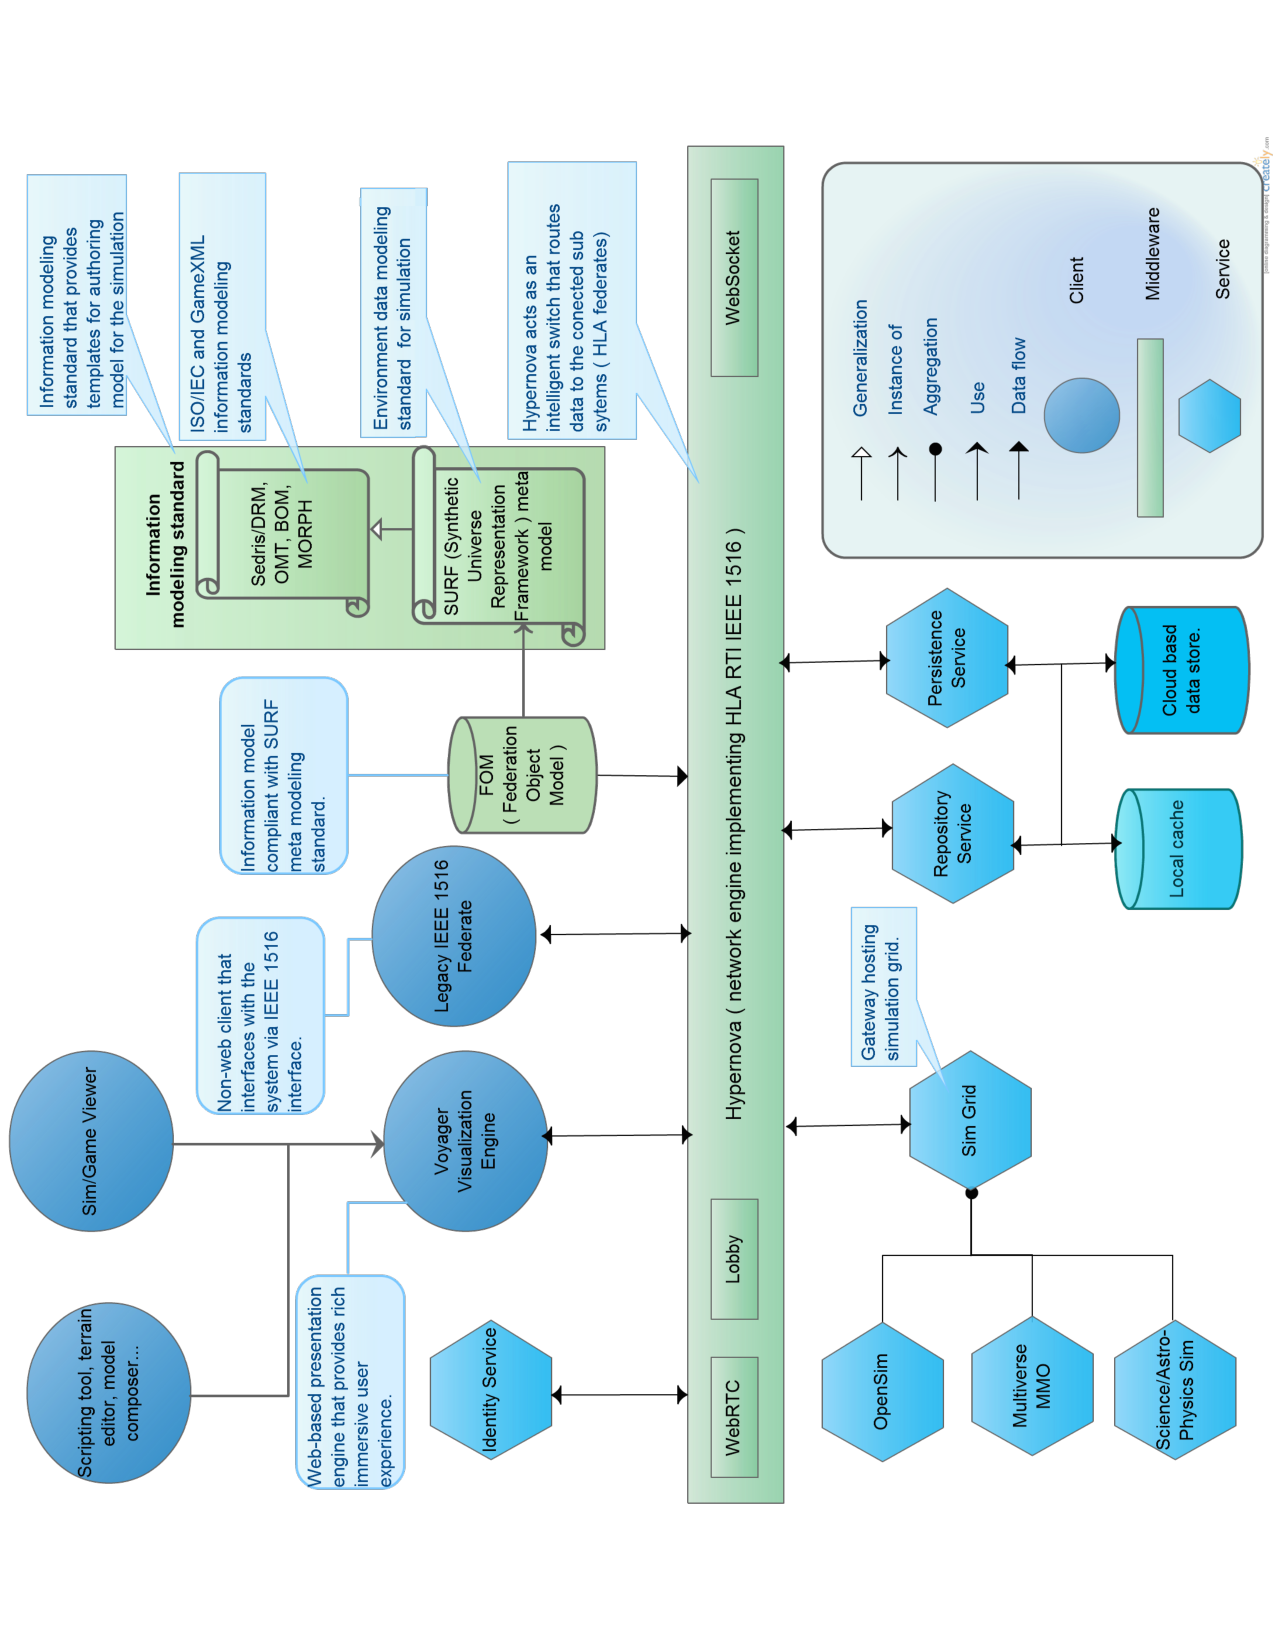
\includegraphics[height=\textwidth,angle=-90]{Arch2.pdf}
  \caption{Potential Interoperability Architecture for the CHORUS Software Platform}
\end{figure}
